\chapterimage{MathCover.png}
\chapter{Water Math - Week 2}



\begin{table}[H]
\begin{tabular}{| m{1cm} | m{1cm} | m{12cm} |}
\hline
\multicolumn{3}{|l|}{\textbf{Expected   Range of Knowledge for Math}}                                                                      \\ \hline
\multicolumn{3}{|l|}{\textit{Water   Distribution System Operator License Exams}}                                                          \\ \hline
\multicolumn{1}{l|}{} & \multicolumn{1}{l|}{D1-D5} & Ability to calculate   flow rates for a storage facility                     \\ \cline{2-3} 
\multicolumn{1}{l|}{} & \multicolumn{1}{l|}{D1-D5} & Ability to calculate   the volume of a storage facility                      \\ \cline{2-3} 
\multicolumn{1}{l|}{} & \multicolumn{1}{l|}{D1-D5} & Knowledge of unit   conversions                                              \\ \cline{2-3} 
\multicolumn{1}{l|}{} & \multicolumn{1}{l|}{D1-D5} & Ability to calculate   flow rates                                            \\ \cline{2-3} 
\multicolumn{1}{l|}{} & \multicolumn{1}{l|}{D1-D5} & Ability to calculate   pipe volumes                                          \\ \cline{2-3} 
\multicolumn{1}{l|}{} & \multicolumn{1}{l|}{D1-D5} & Ability to calculate   the area of a pipe cross-section                      \\ \cline{2-3}
\multicolumn{1}{l|}{} & \multicolumn{1}{l|}{D1-D5} & Ability to calculate   the volume of a trench                                \\ \cline{2-3}  
\multicolumn{1}{l|}{} & \multicolumn{1}{l|}{D1-D5} & Ability to calculate   the surface area of a valve face                      \\ \cline{2-3} 
\multicolumn{1}{l|}{} & \multicolumn{1}{l|}{D1-D5} & Ability to calculate   the volume of a cylinder, rectangle, and square       \\ \cline{2-3} 
\multicolumn{1}{l|}{} & \multicolumn{1}{l|}{D1-D5} & Ability to calculate   the volume of a pipe                                  \\ \cline{2-3} 
\multicolumn{1}{l|}{} & \multicolumn{1}{l|}{D1-D5} & Ability to calculate   the volume of a well, storage reservoir, pipe, trench \\ \cline{2-3} 
\multicolumn{1}{l|}{} & \multicolumn{1}{l|}{D1-D5} & Ability to calculate   the well draw down                                    \\ \cline{2-3} 
\multicolumn{1}{l|}{} & \multicolumn{1}{l|}{D1-D5} & Ability to calculate   total force on a valve                                \\ \cline{2-3} 
\multicolumn{1}{l|}{} & \multicolumn{1}{l|}{D1-D5} & Ability to convert   pressure to feet of head                                \\ \cline{2-3} 
\multicolumn{1}{l|}{} & \multicolumn{1}{l|}{D1-D5} & Ability to convert   units of volume, area, and time                         \\ \cline{2-3} 
\multicolumn{1}{l|}{} & \multicolumn{1}{l|}{D1-D5} & Ability to convert   units of volume, area, pressure, and time               \\ \cline{2-3} 
\multicolumn{1}{l|}{} & \multicolumn{1}{l|}{D1-D5} & Ability to convert   units of volume, pressure and area                      \\ \cline{2-3} 
\multicolumn{1}{l|}{} & \multicolumn{1}{l|}{D1-D5} & Ability to convert   water units                                             \\ \cline{2-3} 
\multicolumn{1}{l|}{} & \multicolumn{1}{l|}{D2-D5} & Ability to calculate   pipe capacity                                         \\ \cline{2-3} 
\multicolumn{1}{l|}{} & \multicolumn{1}{l|}{D2-D5} & Ability to calculate   the velocity of water                                 \\ \cline{2-3} 
\multicolumn{1}{l|}{} & \multicolumn{1}{l|}{D2-D5} & Ability to calculate   thrust block size                                     \\ \cline{2-3} 
\multicolumn{1}{l|}{} & \multicolumn{1}{l|}{D2-D5} & Ability to convert a   pressure reading to depth of water                    \\ \cline{2-3} 
\multicolumn{1}{l|}{} & \multicolumn{1}{l|}{D2-D5} & Ability to convert a   scale to actual distance                              \\ \cline{2-3} 
\end{tabular}
\end{table}
\newpage






\begin{table}[H]
\begin{tabular}{| m{1cm} | m{1cm} | m{12cm} |}
\hline
\multicolumn{3}{|l|}{\textbf{Expected   Range of Knowledge for Math}}                                                                      \\ \hline
\multicolumn{3}{|l|}{\textit{Water   Distribution System Operator License Exams (Continued)}}                                                          \\ \hline
\multicolumn{1}{l|}{} & \multicolumn{1}{l|}{D3-D5} & Ability to calculate   brake-horsepower                                      \\ \cline{2-3} 
\multicolumn{1}{l|}{} & \multicolumn{1}{l|}{D3-D5} & Ability to calculate   pump efficiency                                       \\ \cline{2-3} 
\multicolumn{1}{l|}{} & \multicolumn{1}{l|}{D3-D5} & Ability to calculate   specific yield of a well                              \\ \cline{2-3} 
\multicolumn{1}{l|}{} & \multicolumn{1}{l|}{D3-D5} & Ability to calculate   the cost of water production                          \\ \cline{2-3} 
\multicolumn{1}{l|}{} & \multicolumn{1}{l|}{D4-D5} & Ability to calculate a water loss rate                                       \\ \cline{2-3} 
\multicolumn{1}{l|}{} & \multicolumn{1}{l|}{D4-D5} & Ability to calculate the cost of pumping   water                             \\ \cline{2-3} 
\multicolumn{1}{l|}{} & \multicolumn{1}{l|}{D4-D5} & Ability to calculate the hydraulic gradient                                  \\ \cline{2-3} 
\multicolumn{1}{l|}{} & \multicolumn{1}{l|}{D4-D5} & Ability to calculate water production costs                                  \\ \hline
\multicolumn{3}{|l|}{Water   Treatment Operator License Exams}                                                                    \\ \hline
\multicolumn{1}{l|}{} & \multicolumn{1}{l|}{T1-T4} & Ability to calculate   flow rates and water velocity                         \\ \cline{2-3} 
\multicolumn{1}{l|}{} & \multicolumn{1}{l|}{T1-T4} & Ability to calculate   the volume of water in a storage facility             \\ \cline{2-3} 
\multicolumn{1}{l|}{} & \multicolumn{1}{l|}{T1-T4} & Ability to calculate   well head pressure                                    \\ \cline{2-3} 
\multicolumn{1}{l|}{} & \multicolumn{1}{l|}{T1-T4} & Ability to convert   common water units (e.g. gallons per minute to MGD)     \\ \cline{2-3} 
\multicolumn{1}{l|}{} & \multicolumn{1}{l|}{T1-T4} & Ability to convert   head pressure to water elevation                        \\ \cline{2-3} 
\multicolumn{1}{l|}{} & \multicolumn{1}{l|}{T1-T4} & Ability to convert   units of length, volume, flow and pressure              \\ \cline{2-3} 
\multicolumn{1}{l|}{} & \multicolumn{1}{l|}{T1-T4} & Ability to determine   water level in a storage tank, reservoir, or well     \\ \cline{2-3} 
\multicolumn{1}{l|}{} & \multicolumn{1}{l|}{T1-T4} & Ability to calculate   a chemical dosage                                     \\ \cline{2-3} 
\multicolumn{1}{l|}{} & \multicolumn{1}{l|}{T1-T4} & Ability to calculate   a chemical solution concentration                     \\ \cline{2-3} 
\multicolumn{1}{l|}{} & \multicolumn{1}{l|}{T1-T4} & Ability to calculate   chlorine demand and chlorine residual                 \\ \cline{2-3} 
\multicolumn{1}{l|}{} & \multicolumn{1}{l|}{T1-T4} & Ability to convert   common water units, (gallons per minute to MGD, etc...) \\ \cline{2-3} 
\multicolumn{1}{l|}{} & \multicolumn{1}{l|}{T1-T4} & Ability to determine   water level in a storage tank, reservoir or well      \\ \cline{2-3} 
\multicolumn{1}{l|}{} & \multicolumn{1}{l|}{T3-T4} & Ability to perform   blending calculations                                   \\ \cline{2-3} 
\multicolumn{1}{l|}{} & \multicolumn{1}{l|}{T3-T4} & Ability to calculate   a dilution factor                                     \\ \cline{2-3} 
\multicolumn{1}{l|}{} & \multicolumn{1}{l|}{T3-T4} & Ability to mix   chemicals and prepare reagents                              \\ \cline{2-3} 
\multicolumn{1}{l|}{} & \multicolumn{1}{l|}{T3-T4} & Ability to perform   dilutions                                               \\ \cline{2-3} 
\multicolumn{1}{l|}{} & \multicolumn{1}{l|}{T3-T4} & Ability to calculate   a coagulant dose from a jar test                      \\ \cline{2-3} 
\multicolumn{1}{l|}{} & \multicolumn{1}{l|}{T3-T4} & Ability to calculate   a filter-aid dosage                                   \\ \cline{2-3} 
\multicolumn{1}{l|}{} & \multicolumn{1}{l|}{T3-T4} & Ability to calculate   a filtration rate                                     \\ \cline{2-3} 
\multicolumn{1}{l|}{} & \multicolumn{1}{l|}{T3-T4} & Ability to calculate   filter loading rate                                   \\ \cline{2-3} 
\multicolumn{1}{l|}{} & \multicolumn{1}{l|}{T3-T4} & Ability to calculate   percent or log removal of contaminants from water     \\ \cline{2-3} 
\multicolumn{1}{l|}{} & \multicolumn{1}{l|}{T3-T4} & Ability to calculate   the cost of water treatment operations                \\ \cline{2-3} 
\end{tabular}
\end{table}
\newpage



\section{Working with Percent}\index{Working with Percent}
\begin{itemize}
\item Percent expresses portions of the whole.  
\item \texthl{The whole is considered as 1 or 100\% and a part of the whole can be expressed as a percent.}
\textbf{Example:} If a tank is $1 / 2$ full, we say that it contains $50 \%$ of the original solution.
\item Percentage is written as a whole number with a \% sign after it. 
\item In a calculation, percent is expressed as a decimal. 
\item \texthl{The decimal form of a percent value is obtained by dividing the percent by 100.}\\
 \textbf{Example:} $11 \%$ is expressed as the decimal $0.11$, since $11 \%$ is equal to $11 / 100$. This decimal is obtained by dividing 11 by 100.
\item \texthl{To determine what percentage a part is of the whole, divide the part by the whole.}\\
\textbf{Example:} There are 80 water meters to read, Jim has finished 24 of them. What percentage of the meters have been read?\\
$$24 \div 80=0.30$$\\
The $0.30$ is converted to percent by multiplying the answer by 100.\\
$$0.30 \times 100=30 \%$$\\
Thus $30 \%$ of the 80 meters have been read.\\

\item \texthl{To find the percentage of a number, multiply the number by the decimal equivalent of the percentage given in the problem.}\\
\textbf{Example:}\\
What is $28 \%$ of $286 ?$\\

\begin{enumerate}[Step 1.]
\item Change the $28 \%$ to a decimal equivalent:  $$28 \% \div 100=0.28$$
\item Multiply $286 \times 0.28=80$\\
Thus $28 \%$ of 286 is 80.
\end{enumerate}

\item \texthl{To increase a value by a percent, add the decimal equivalent of the percent to " 1 " and multiply it times the number.}

\textbf{Example:} A filter bed will expand $25 \%$ during backwash. If the filter bed is 36 inches deep, how deep will it be during backwash?\\

\begin{enumerate}[Step 1.]
\item Change the percent to a decimal.
$$
25 \% \div 100=0.25
$$
\item Add the whole number 1 to this value.
$$
1+0.25=1.25
$$
\item Multiply times the value.
$$
36 \text { in } \times 1.25=45 \text { inches }
$$
\end{enumerate}
\end{itemize}




% \begin{tcolorbox}[
% colframe=blue!25,
% colback=blue!10,
% coltitle=blue!20!black,  
% title= Practice Problems]
% \begin{enumerate}
% \item $25 \%$ of the chlorine in a 30-gallon vat has been used. How many gallons are remaining in the vat?

% \item The annual public works budget is $\$ 147,450$. If $75 \%$ of the budget should be spent by the end of September, how many dollars are to be spent? How many dollars will be remaining?

% \item A 75 pound container of calcium hypochlorite has a purity of $67 \%$. What is the total weight of the calcium hypochlorite? 

% \item $3 / 4$ is the same as what percentage?

% \end{enumerate}
% \end{tcolorbox}









\section{Area \& Volume}\index{Area \& Volume}
% \section{Area \& Volume}\index{Area \& Volume}

% \begin{snugshade*}
% 	\item \noindent\textsc{Area \& Volume}
% \end{snugshade*}

\begin{center}
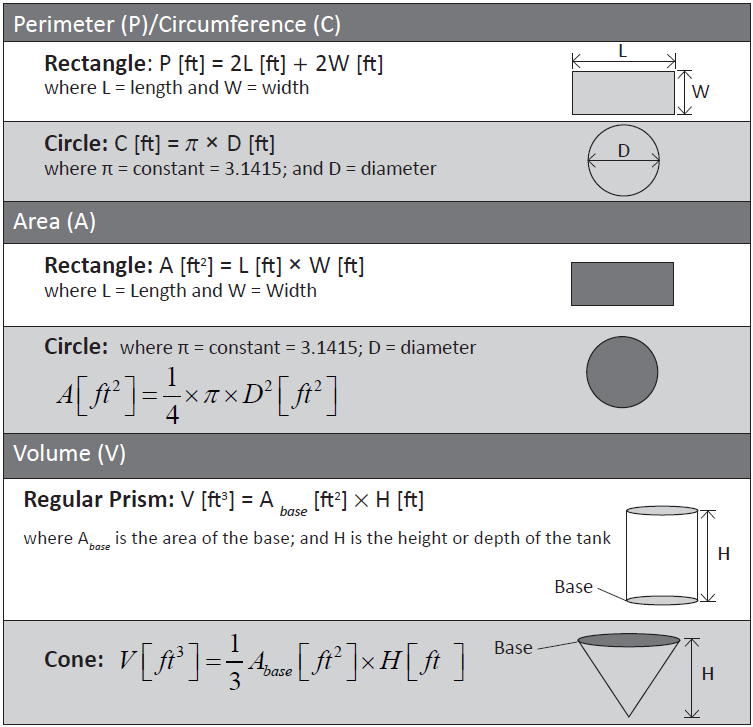
\includegraphics[scale=0.5]{Area&VolumeFormula}
\end{center}
\textbf{Example 1:} The floor of a rectangular building is 20 feet long by 12 feet wide and the inside walls are 10 feet high. Find the total surface area of the inside walls of this building\\
Solution:\\
% \begin{center}
\begin{tikzpicture}
	%%% Edit the following coordinate to change the shape of your
	%%% cuboid
      
	%% Vanishing points for perspective handling
	\coordinate (P1) at (-7cm,1.5cm); % left vanishing point (To pick)
	\coordinate (P2) at (8cm,1.5cm); % right vanishing point (To pick)

	%% (A1) and (A2) defines the 2 central points of the cuboid
	\coordinate (A1) at (0em,0cm); % central top point (To pick)
	\coordinate (A2) at (0em,-2cm); % central bottom point (To pick)

	%% (A3) to (A8) are computed given a unique parameter (or 2) .8
	% You can vary .8 from 0 to 1 to change perspective on left side
	\coordinate (A3) at ($(P1)!.8!(A2)$); % To pick for perspective 
	\coordinate (A4) at ($(P1)!.8!(A1)$);

	% You can vary .8 from 0 to 1 to change perspective on right side
	\coordinate (A7) at ($(P2)!.7!(A2)$);
	\coordinate (A8) at ($(P2)!.7!(A1)$);

	%% Automatically compute the last 2 points with intersections
	\coordinate (A5) at
	  (intersection cs: first line={(A8) -- (P1)},
			    second line={(A4) -- (P2)});
	\coordinate (A6) at
	  (intersection cs: first line={(A7) -- (P1)}, 
			    second line={(A3) -- (P2)});

	%%% Depending of what you want to display, you can comment/edit
	%%% the following lines

	%% Possibly draw back faces

	\fill[gray!40] (A2) -- (A3) -- (A6) -- (A7) -- cycle; % face 6
	\node at (barycentric cs:A2=1,A3=1,A6=1,A7=1) {\tiny Floor=W*L};
	
	\fill[gray!50] (A3) -- (A4) -- (A5) -- (A6) -- cycle; % face 3
	\node at (barycentric cs:A3=1,A4=1,A5=1,A6=1) {\tiny Wall - W*H};
	
	\fill[gray!10, opacity=0.2] (A5) -- (A6) -- (A7) -- (A8) -- cycle; % face 4
	\node at (barycentric cs:A5=1,A6=1,A7=1,A8=1) {\tiny Wall - L*H};
	
	\fill[gray!10,opacity=0.5] (A1) -- (A2) -- (A3) -- (A4) -- cycle; % f2
	\node at (barycentric cs:A1=1,A2=1,A3=1,A4=1) {\tiny Wall - L*H};
	
	\fill[gray!40,opacity=0.2] (A1) -- (A4) -- (A5) -- (A8) -- cycle; % f5
	\node at (barycentric cs:A1=1,A4=1,A5=1,A8=1) {\tiny Ceiling=W*L};	
	
	\draw[thick,dashed] (A5) -- (A6);
	\draw[thick,dashed] (A3) -- (A6);
	\draw[thick,dashed] (A7) -- (A6);

	%% Possibly draw front faces

	%\fill[orange] (A1) -- (A8) -- (A7) -- (A2) -- cycle; % face 1
	\node at (barycentric cs:A1=1,A8=1,A7=1,A2=1) {\tiny Wall - W*H};
	


	%% Possibly draw front lines
	\draw[thick] (A1) -- (A2);

	\draw[<->] (-1.8,0.38) -- (-1.8,-1.3)node [midway, above=-1.8mm] {\hspace{-1.3cm}\tiny Height=10'};
	\draw[<->] (-1.6,-1.4) -- (-.3,-2.1)node [midway, above=-2.6mm] {\hspace{-1.3cm}\tiny Length=20'};
	\draw[<->] (2.6,-1.13) -- (0.2,-2.2)node [midway, below=.6mm] {\hspace{1.2cm}\tiny Width=12'};
	\draw[thick] (A3) -- (A4);
	\draw[thick] (A7) -- (A8);
	\draw[thick] (A1) -- (A4);
	\draw[thick] (A1) -- (A8);
	\draw[thick] (A2) -- (A3);
	\draw[thick] (A2) -- (A7);
	\draw[thick] (A4) -- (A5);
	\draw[thick] (A8) -- (A5);
	
	% Possibly draw points
	% (it can help you understand the cuboid structure)
%	\foreach \i in {1,2,...,8}
%	{
%	  \draw[fill=black] (A\i) circle (0.15em)
%	    node[above right] {\tiny \i};
%	}
	% \draw[fill=black] (P1) circle (0.1em) node[below] {\tiny p1};
	% \draw[fill=black] (P2) circle (0.1em) node[below] {\tiny p2};
\end{tikzpicture}\\
% \end{center}
2 Walls W*H + 2 Walls L*H= $2*12*10ft^2 + 2*20*10ft^2$\\
$=240+400=\boxed{640ft^2}$\\

2 Walls W*H + 2 Walls L*H + Floor + Ceiling= $2*12*10ft^2 + 2*20*10ft^2 + 2*12*20ft^2$\\
$=240+400+480=\boxed{1,120ft^2}$\\

\textbf{Example 2:} How many gallons of paint will be required to paint the inside walls of a 40 ft long x 65 ft wide x 20 ft high tank if the paint coverage is 150 sq. ft per gallon.  Note:  We are painting walls only.  Disregard the floor and roof areas.\\
Solution:\\
\vspace{0.3cm}
% \begin{center}
\begin{tikzpicture}
	%%% Edit the following coordinate to change the shape of your
	%%% cuboid
      
	%% Vanishing points for perspective handling
	\coordinate (P1) at (-7cm,1.5cm); % left vanishing point (To pick)
	\coordinate (P2) at (8cm,1.5cm); % right vanishing point (To pick)

	%% (A1) and (A2) defines the 2 central points of the cuboid
	\coordinate (A1) at (0em,0cm); % central top point (To pick)
	\coordinate (A2) at (0em,-2cm); % central bottom point (To pick)

	%% (A3) to (A8) are computed given a unique parameter (or 2) .8
	% You can vary .8 from 0 to 1 to change perspective on left side
	\coordinate (A3) at ($(P1)!.8!(A2)$); % To pick for perspective 
	\coordinate (A4) at ($(P1)!.8!(A1)$);

	% You can vary .8 from 0 to 1 to change perspective on right side
	\coordinate (A7) at ($(P2)!.7!(A2)$);
	\coordinate (A8) at ($(P2)!.7!(A1)$);

	%% Automatically compute the last 2 points with intersections
	\coordinate (A5) at
	  (intersection cs: first line={(A8) -- (P1)},
			    second line={(A4) -- (P2)});
	\coordinate (A6) at
	  (intersection cs: first line={(A7) -- (P1)}, 
			    second line={(A3) -- (P2)});

	%%% Depending of what you want to display, you can comment/edit
	%%% the following lines

	%% Possibly draw back faces

	\fill[gray!40] (A2) -- (A3) -- (A6) -- (A7) -- cycle; % face 6
	\node at (barycentric cs:A2=1,A3=1,A6=1,A7=1) {};
	
	\fill[gray!50] (A3) -- (A4) -- (A5) -- (A6) -- cycle; % face 3
	\node at (barycentric cs:A3=1,A4=1,A5=1,A6=1) {\tiny Wall - W*H};
	
	\fill[gray!10, opacity=0.2] (A5) -- (A6) -- (A7) -- (A8) -- cycle; % face 4
	\node at (barycentric cs:A5=1,A6=1,A7=1,A8=1) {\tiny Wall - L*H};
	
	\fill[gray!10,opacity=0.5] (A1) -- (A2) -- (A3) -- (A4) -- cycle; % f2
	\node at (barycentric cs:A1=1,A2=1,A3=1,A4=1) {\tiny Wall - L*H};
	
	\fill[gray!40,opacity=0.2] (A1) -- (A4) -- (A5) -- (A8) -- cycle; % f5
	\node at (barycentric cs:A1=1,A4=1,A5=1,A8=1) {};	
	
	\draw[thick,dashed] (A5) -- (A6);
	\draw[thick,dashed] (A3) -- (A6);
	\draw[thick,dashed] (A7) -- (A6);

	%% Possibly draw front faces

	%\fill[orange] (A1) -- (A8) -- (A7) -- (A2) -- cycle; % face 1
	\node at (barycentric cs:A1=1,A8=1,A7=1,A2=1) {\tiny Wall - W*H};
	


	%% Possibly draw front lines
	\draw[thick] (A1) -- (A2);

	\draw[<->] (-1.8,0.38) -- (-1.8,-1.3)node [midway, above=-1.8mm] {\hspace{-1.3cm}\tiny Height=20'};
	\draw[<->] (-1.6,-1.4) -- (-.3,-2.1)node [midway, above=-2.6mm] {\hspace{-1.3cm}\tiny Length=40'};
	\draw[<->] (2.6,-1.13) -- (0.2,-2.2)node [midway, below=.6mm] {\hspace{1.2cm}\tiny Width=65'};
	\draw[thick] (A3) -- (A4);
	\draw[thick] (A7) -- (A8);
	\draw[thick] (A1) -- (A4);
	\draw[thick] (A1) -- (A8);
	\draw[thick] (A2) -- (A3);
	\draw[thick] (A2) -- (A7);
	\draw[thick] (A4) -- (A5);
	\draw[thick] (A8) -- (A5);
	
	% Possibly draw points
	% (it can help you understand the cuboid structure)
%	\foreach \i in {1,2,...,8}
%	{
%	  \draw[fill=black] (A\i) circle (0.15em)
%	    node[above right] {\tiny \i};
%	}
	% \draw[fill=black] (P1) circle (0.1em) node[below] {\tiny p1};
	% \draw[fill=black] (P2) circle (0.1em) node[below] {\tiny p2};
\end{tikzpicture}\\
% \end{center}
\vspace{0.3cm}
2 Walls W*H + 2 Walls L*H = $2*65*20ft^2 + 2*40*20ft^2= 2,600+1,600=4,200ft^2$\\
$\implies @150\dfrac{ft^2}{gal} \enspace paint \enspace coverage \enspace \rightarrow \enspace \dfrac{4,200\cancel{ft^2}}{150\dfrac{\cancel{ft^2}}{gal}}=\boxed{28 \enspace gallons}$
\vspace{0.3cm}
\textbf{Example 3:}  What is the circumference of a 100 ft diameter circular sedimentation tank?\\
\vspace{0.3cm}
Solution:\\
\vspace{0.3cm}
$Circumference=\pi*D=3.14*100ft=\boxed{314ft}$
\vspace{0.3cm}

\textbf{Example 4:} If the surface area of a clarifier is 5,025$ft^2$, what is its diameter?\\
\vspace{0.3cm}
Solution:\\
\vspace{0.3cm}
$Surface \enspace area=\dfrac{\pi}{4}*D^2 \enspace \implies 5025(ft^2)=0.785*D^2 (ft^2)$\\
$\implies D^2=\dfrac{5025}{0.785} \implies D=\sqrt{6401.3}=\boxed{80ft}$
\vspace{0.3cm}

\textbf{Example 5:} How many gallons of water would 600 feet of 6-inch diameter pipe hold, approximately?\\
\vspace{0.3cm}
Solution:\\

\vspace{0.3cm}
% \begin{center}
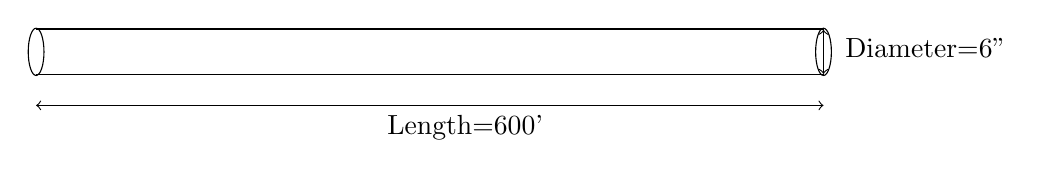
\begin{tikzpicture}
\draw (0,0) ellipse (0.1cm and 0.3cm);
\draw (10,0) ellipse (0.1cm and 0.3cm);
\draw [-] (0,-0.29) -- (10,-0.29);
\draw [-] (0,0.29) -- (10,0.29);
\draw [<->] (10,-0.28) -- (10,0.28) node [midway, below=-3mm] {\hspace{2.6cm}Diameter=6"};
\draw [<->] (0,-.68) -- (10,-.68)node [midway, below] {\hspace{0.9cm}Length=600'};
\end{tikzpicture}
% \end{center}
\vspace{0.3cm}
$Volume=\dfrac{\pi}{4}D^2*L=0.785*\Big(\dfrac{6}{12}\Big)^2*600\cancel{ft^3}*7.48\dfrac{gallons}{\cancel{ft^3}}=\boxed{881 \enspace gallons}$

% \begin{tcolorbox}[
% colframe=blue!25,
% colback=blue!10,
% coltitle=blue!20!black,  
% title= Practice Problems]
% \begin{enumerate}

% \item A 60-foot diameter tank contains 422,000 gallons of water. Calculate the height of water in the storage tank.

% \item What is the volume of water in ft$^3$, of a sedimentation basin that is 22 feet long, and 15 feet wide, and filled to 10 feet?

% \item What is the volume in ft$^3$ of an elevated clear well that is 17.5 feet in diameter, and filled to 14 feet?

% \item What is the area of the top of a storage tank that is 75 feet in diameter?\\

% \item  What is the area of a wall $175 \mathrm{ft}$. in length and $20 \mathrm{ft}$. wide?\\

% \item  You are tasked with filling an area with rock near some of your equipment. 1 Bag of rock covers 250 square feet. The area that needs rock cover is 400 feet in length and 30 feet wide. How many bags do you need to purchase?\\
% \end{enumerate}
% \end{tcolorbox}

\section{Flow and Velocity}\index{Flow and Velocity}
\begin{itemize}
\item Flow Rate - Q (volume/time) = velocity (distance or length traveled /time) * surface area
\item Velocity is the speed at which the water is flowing.  It is measured in units of length/time – ft./sec.
\item Velocity of water flowing through can be calculated by dividing the flow rate by area of the flow stream.\\
\vspace{0.5cm}
$$Velocity \enspace \dfrac{length}{time}= \dfrac{flow \enspace rate(\dfrac{volume \enspace or \enspace cubic \enspace length}{time})}{surface \enspace area \enspace in \enspace the \enspace direction \enspace of \enspace flow-square \enspace length}$$
\vspace{0.5cm}
\textbf{For a flow in a channel:}\\
\vspace{0.5cm}
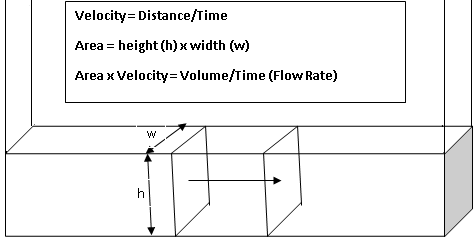
\includegraphics[scale=0.5]{ChannelFlow3}\\

\textbf{For a flow in a pipe:}\\
\vspace{0.5cm}
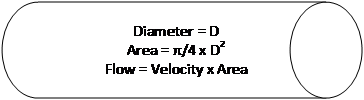
\includegraphics[scale=0.65]{VelocityinPipe}\\
\vspace{0.5cm}
\end{itemize}
\subsection*{Example Problems}
\textbf{Example:} If a chemical is added in a pipe where water is flowing at a velocity of 3.1 feet per second, how many minutes would it take for the chemical to reach a point 7 miles away?  \\

Note - we want the answer in minutes\\

$$\textrm{Min } = \dfrac{1}{3.1}\dfrac{sec}{ft}*\dfrac{5280ft}{mile}*7 miles*\dfrac{min}{60 sec} = \boxed{199 min}$$
\\

\textbf{Example:} Find the flow in cfs in a 6 -inch line, if the velocity is 2 feet per second.

\begin{enumerate}
\item Determine the cross-sectional area of the line in square feet. Start by converting the diameter of the pipe to inches.

The diameter is 6 inches: therefore, the radius is 3 inches. 3 inches is $3 / 12$ of a foot or $0.25$ feet.

\item Now find the area in square feet.
$$
\begin{aligned}
&A=\pi \times r^{2} \\
&A=\pi \times\left(0.25 \mathrm{ft}^{2}\right. \\
&A=\pi \times 0.0625 \mathrm{ft}^{2} \\
&A=0.196 \mathrm{ft}^{2}
\end{aligned}
$$
Or
$$
\begin{aligned}
&A=0.785 \times D^{2} \\
&A=0.785 \times 0.5^{2} \\
&A=0.785 \times .05 \times .05 \\
&A=0.196 \mathrm{ft}^{2}
\end{aligned}
$$

\item Now find the flow.

$\mathrm{Q}=\mathrm{V} \times \mathrm{A}$

$\mathrm{Q}=2 \mathrm{ft} / \mathrm{sec} \times 0.196 \mathrm{ft}^{2}$

$\mathrm{Q}=0.3927 \mathrm{cfs}$ or $0.4 \mathrm{cfs}$

\end{enumerate}


\textbf{Example:} A rectangular channel 3 ft. wide contains water 2 ft. deep flowing at a velocity of 1.5 fps.
What is the flow rate in cfs?

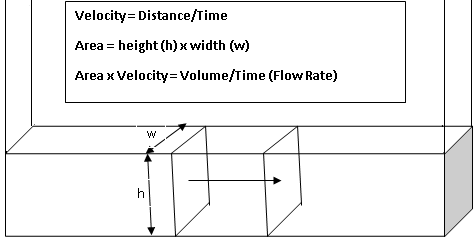
\includegraphics[scale=0.5]{ChannelFlow3}\\
$Q=V*A \implies Q = 1.5 \dfrac{ft}{sec}*(3*2)ft^2=\boxed{9\dfrac{ft^3}{sec}}$

\vspace{1cm}

% \begin{tcolorbox}[
% colframe=blue!25,
% colback=blue!10,
% coltitle=blue!20!black,  
% title= Practice Problems]
% \begin{enumerate}

% \item Flow in an 8-inch pipe is 500 gpm. What is the average velocity in ft/sec? (Assume pipe is flowing full)

% \item A pipeline is 18” in diameter and flowing at a velocity of 125 ft. per minute. What is the flow in gallons per minute?

% \item The velocity in a pipeline is 2 ft./sec. and the flow is 3,000 gpm. What is the diameter of the pipe in inches?



% \item Find the flow in a 4-inch pipe when the velocity is $1.5$ feet per second.

%   \item A 42-inch diameter pipe transfers 35 cubic feet of water per second. Find the velocity in $\mathrm{ft} / \mathrm{sec}$. 
  
%   \item A plastic float is dropped into a channel and is found to travel 10 feet in $4.2$ seconds. The channel is $2.4$ feet wide and $1.8$ feet deep. Calculate the flow rate of water in cfs.
%   \end{enumerate}
%   \end{tcolorbox}

\section{Contaminant Removal Efficiency}\index{Contaminant Removal Efficiency}
\begin{itemize}
\item Contaminant removal efficiency can be expressed as the percentage of the inlet concentration removed and can be established based upon the amount of a particular contaminant entering and leaving a treatment process.

\item $Percent \enspace Removal \enspace (\%) = \dfrac{Concentration \enspace  In-Concentration\enspace  Out}{Concentration \enspace In}*100$\\

\item If 10 units of a contaminant are entering a process and 8 units of pollutant are leaving (process removes 2 units), then the process removal rate for that pollutant is (10-8)/10*100=20\%.  In this example the process is 20\% efficient in removing that particular contaminant.

\item Besides percent removal, removal efficiency can also be expressed in terms of Log removal.
\item Background of log:\\ 
Log of a number $x$ to the \textbf{base} $B$ is the exponent to which $B$ must be \textbf{raised} to produce $x$.\\
\vspace{0.3cm}
\begin{center}
$\log_B x=A \implies B^A=x$\\
For Example: $\log_{10} 1000=3 \implies 10^3=1000$ \\
\end{center}
\vspace{0.3cm}
Log Rules\\
\begin{enumerate}
\item $\log_{b} 1=0$
\item $\log_{b} ac=\log_{b} a + \log_{b} c$
\item $\log_{b} \dfrac{a}{c}=\log_{a} a - \log_{b} c$
\item $\log_{b} a^r=r\log_{b} a$
\item $\log_{b} \dfrac{1}{c}=-\log_{b} c$
\end{enumerate}
\vspace{0.3cm}
\item Log removal is:  $\log_{10} {(Concentration \enspace In)} - \log_{10} {(Concentration \enspace Out)}$
\item \textbf{CASE 1: } Say the initial (before treatment) and final (after treatment) cryptosporidium concentrations are 100 oocysts and 10 oocysts per L respectively. \\
\vspace{0.3cm}
Thus log removal is $\log_{10} 100 - \log_{10} 10 = \log_{10}\dfrac{100}{10}=\log_{10} 10 = \boxed{1} \enspace as \enspace 10^1=10 $\\
\vspace{0.3cm}
\item The removal on a percentage basis: $\mathrm{Percent \enspace removal} = \dfrac{\mathrm{initial}-\mathrm{final}}{\mathrm{intial}}*100=\dfrac{100-10}{100}*100=90\%$\\
\item \textbf{CASE 2: } Say the initial (before treatment) and final (after treatment) cryptosporidium concentrations are 100 oocysts and 1 oocysts per L respectively. \\
\vspace{0.3cm}
Thus log removal is $\log_{10} 100 - \log_{10} 1 = \log_{10}\dfrac{100}{1}=\log_{10} 100 = \boxed{2} \enspace as \enspace 10^2=100 $\\
\vspace{0.3cm}
\item The removal on a percentage basis: $\mathrm{Percent \enspace removal} = \dfrac{\mathrm{initial}-\mathrm{final}}{\mathrm{intial}}*100=\dfrac{100-1}{100}*100=99\%$\\
\vspace{0.5cm}
\item \textbf{CASE 3: } If the initial (before treatment) and final (after treatment) cryptosporidium concentrations are 1000 oocysts and 1 oocysts per L respectively. (unreal values....) \\
\vspace{0.3cm}
Thus log removal is $\log_{10} 1000 - \log_{10} 10 = \log_{10}\dfrac{1000}{1}=\log_{10} 1000 = \boxed{3} \enspace as \enspace 10^3=1000 $\\
\vspace{0.3cm}
The removal on a percentage basis: $\mathrm{Percent \enspace removal} = \dfrac{\mathrm{initial}-\mathrm{final}}{\mathrm{intial}}*100=\dfrac{1000-1}{1000}*100=99.9\%$
\vspace{0.3cm}
\item Thus:\\
1 log removal =90\% removal efficiency\\
2 log removal =99\% removal efficiency\\
3 log removal =99.9\% removal efficiency\\
4 log removal =99.99\% removal efficnecy\\
\end{itemize}
